\chapter{Auswertung}
\label{cha:auswertung}

In diesem Kapitel: //TODO Einführung in das Kapitel

\section{Konvergenz des TD-Q-Lernens}

\subsection{Generalisierung oder Funktionsannäherung}
\label{subsec:Generalisierung oder Funktionsannäherung}

\paragraph{Samuels Dame-Spiel}
Arthur L. Samuel schrieb 1955 ein Programm, dass Dame spielen konnte und mit einem einfachen Lernverfahren seine Parameter verbessern konnte. Sein Programm hatte dabei jedoch Zugriff auf eine große Zahl von archivierten Spielen, bei denen jeder einzelne Zug von Experten bewertet war (Überwachtes Lernen zur Unterstützung des verstärkenden Lernens). Damit verbesserte das Programm seine Bewertungsfunktion. Um eine noch weitere Verbesserung zu erreichen, ließ Samuel dein Programm gegen sich selbst spielen. Das Credit Assignment löste er auf einfache Weise. Für jede einzelne Stellung während eines Spiels vergleicht er die Bewertung durch die Funktion B(s) mit der durch Alpha-Beta-Pruning berechneten Bewertung und verändert B(s) entsprechend. 1961 besiegte sein Dame-Programm den viertbesten Damespieler der USA. Mit dieser bahnbrechenden Arbeit war Samuel seiner Zeit um fast dreißig Jahre voraus \cite[120\psq]{Ertel}.

\paragraph{Agent mit TD-Lernen}
Die Aufgabe des Agenten mit TD-Lernen ist, dass verbessern einer gegebenen Heuristik. Unter Verwendung dieser möglicherweise verbesserten Heuristik, soll der Agent eine möglichst optimale Aktion auswählen. Der Agent verbessert die Bewertungsfunktion durch Aktualisierung bzw. Anpassung der Parameter $\theta = \theta_1, ... \theta_n$. 

\begin{equation*}
\hat{U}_\theta(s) = \theta_1 f_1(s) + \theta_2 f_2(s) + ... + \theta_n f_n(s)
\end{equation*}

\subsection{Neuronales Lernen}
\label{subsec:Neuronales Lernen}

\paragraph{TD-Gammon}
Das TD-Lernen zusammen mit einem Backpropagation-Netz mit 40 bis 80 verdeckten Neuronen wurde sehr erfolgreich angewendet in TD-Gammon, einem Programm zum Spielen von Backgammon, programmiert vom Entwickler Gerald Tesauro im Jahr 1992. Die einzige direkte Belohnung für das Programm ist das Ergebnis am Ende eines Spiels. Eine optimierte Version des Programms mit einer 2-Züge-Vorausschau wurde mit 1,5 Millionen Spielen gegen sich selbst trainiert. Es besiegte damit Weltklassespieler und spielt so gut wie die drei besten menschlichen Spieler \cite[304]{Ertel}.  

\paragraph{Sind Lernverfahren überhaupt Sinnvoll?}

\section{Gegenüberstellung der Lernverfahren}
Belastbarkeit und Grenzen der Lernverfahren ? \\
Optimale Anwendungsspiele für die Lernverfahren? \\
Bewertung der Strategien?
\paragraph{Überwachtes Lernen}
\paragraph{Wert-Iteration und dynamische Programmierung}
\paragraph{TD-Lernen}
\paragraph{Q-Lernen}
\paragraph{Funktionsannäherung}


\section{Gegenüberstellung überwachtes und verstärkendes Lernen}
Ein überwachtes Lernverfahren wird zuerst mittels eines Trainingssets kontrolliert belehrt. Das Trainingsset für ein überwachtes Lernverfahren besteht aus verschiedenen Eigenschaften (Features) und einer den Eigenschaften zugeordneten Klasse beziehungsweise Zielvariable (Target variable). Die Qualität der Zielwerte kann mittels Testsets ermittelt werden. Ein Testset ist ein Datenset bestehend aus Eigenschaften ohne die dazugehörigen Klassen. Abbildung \ref{fig:vogel_spezies} zeigt, wie ein Trainingsset aussehen könnte\cite[8]{Harrington}. Die Spalten Gewicht, Flügelspanne, Schwimmhäute und Rückenfarbe sind die Eigenschaften und die Spalte Spezies beinhaltet die Zielvariablen. Das überwachte Lernverfahren lernt mittels des Trainingsdatensets die Beziehungen zwischen den Eigenschaften und der Klassen. \\

\begin{figure}[!htbp]
  \centering
  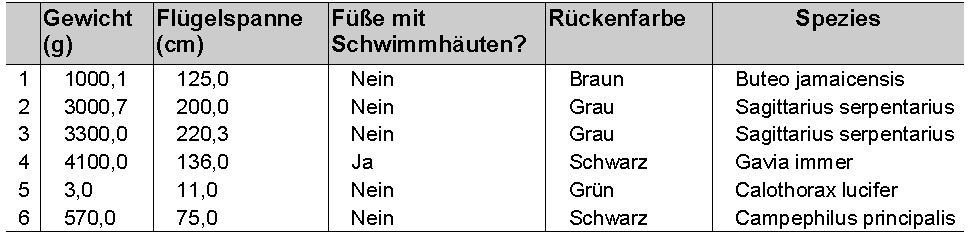
\includegraphics[scale = 0.89]{inhalt/abbildungen/vogel_spezies.pdf}
  \caption{Vogelspezies Klassifikation basierend auf vier Eigenschaften}
  \label{fig:vogel_spezies}
\end{figure} 

Bezogen auf ein Testdatenset wäre eine Aktion des Agenten, dass nennen einer Klasse hinsichtlich der gelernten Zusammenhänge aus den Trainingsdaten. Teilt man die Anzahl der korrekten Vorschläge durch die Anzahl aller Versuche, dann erhält man eine Kennzahl für die Qualität der Vorhersage. Sind alle Klassen der Testinstanzen richtig vorhergesagt, dann ist die Kennzahl genau Eins. Jede Zeile eines Testsets und jede Zeile eines Trainingssets ohne die Zielvariablen ist eine Instanz. \\

Im Gegensatz zu den Lernverfahren beim überwachten Lernen fehlt dem Agenten beim verstärkenden Lernen ein Lehrer (z.B. das Trainingsset), der dem Agenten genau sagt ob seine Aktionen richtig oder falsch sind. Den Experten für Strategiespiele wie Schach fällt es außerdem sehr schwer für jede mögliche Stellung eine angemessen ausformulierte Bewertung bereitzustellen. Zudem ist die Spielzustandsmenge, also die Anzahl an möglichen Stellungen, beim Schach sehr hoch (siehe Abschnitt \ref{subsec:Minimax} Minimax). Selbst wenn es den Experten leicht fallen würde, jede Stellungen explizit bewerten zu können, dann ist die Anzahl der Stellungen immer noch so groß, dass diese Art der Lehre extrem kostspielig wäre. \\

Problembereiche des verstärkenden Lernens sind:
\begin{itemize}
\item Lernen von Problemen mit sehr großen Zustand- und Aktionsmengen
\item Lernen von unbekannten oder sehr komplexen Probleme, für die keine Erfahrungswerte (Testsets) existieren oder diese zu komplex zu beschreiben sind 
\end{itemize}

Verstärkendes Lernen kann trotzdem vom überwachten Lernen profitieren, denn es ist z.B. möglich den Agenten in der Anfangsphase des verstärkten Lernens explizit zu programmieren und ihn dadurch auf bestimmte Auffälligkeiten oder Muster aufmerksam zu machen. Ist es zu kompliziert dies explizit zu programmieren, dann kann auch ein Mensch dem Agenten die richtigen Aktionen vorgeben \cite[306]{Ertel}. \\

Sehr nützlich werden diese beiden Unterstützungen der Anfangsphase des verstärkenden Lernens, sobald die Dimensionen der Umwelt oder des Agenten eine bestimmte Größe überschreiten. Eine Aktionsdimension kann sehr wenige Aktionen beinhalten zum Beispiel die vier Aktionen bewege dich nach oben, unten, rechts oder links. Roboter die dem Menschen nachempfunden sind verfügen über bis zu 50 verschiedene Motoren für die einzelnen Gelenke. Diese müssen gleichzeitig angesteuert werden, was zu einem 50-dimensionalen Zustandsraum und einem 50-dimensionalen Aktionenraum führt\cite[\acs{vgl.} 305\psq]{Ertel}. Bei solch großen Dimensionen können die Laufzeiten einiger verstärkender Lernverfahren massiv ansteigen, bis sie praktisch nicht mehr handhabbar sind. Gerade in der Anfangsphase des verstärkten Lernens kann darum ein Eingriff mittels überwachtem Lernen sehr Laufzeit schonend sein. \\

Zusammengefasst kann das überwachte Lernen die Problematiken des verstärkenden Lernens nicht alleine lösen, aber überwachtes Lernen kann das verstärkende Lernen in bestimmten Lernphasen unterstützen und die Leistung des verstärkenden Lernens verbessern. Später in dieser Arbeit werden wir eine Anwendung betrachten in der unter anderem überwachtes Lernen eingesetzt wurde, um einen verstärkenden Lernalgorithmus zu unterstützen (Samuels Dame-Spiel).